%%%%%%%% ICML 2026 EXAMPLE LATEX SUBMISSION FILE %%%%%%%%%%%%%%%%%

\documentclass{article}

% Recommended, but optional, packages for figures and better typesetting:
\usepackage{microtype}
\usepackage{graphicx}
\usepackage{subcaption}
\usepackage{booktabs} % for professional tables
\usepackage{stfloats}
\usepackage{tikz}
\usetikzlibrary{arrows.meta,positioning}

% hyperref makes hyperlinks in the resulting PDF.
% If your build breaks (sometimes temporarily if a hyperlink spans a page)
% please comment out the following usepackage line and replace
% \usepackage{icml2026} with \usepackage[nohyperref]{icml2026} above.
\usepackage{hyperref}


% Attempt to make hyperref and algorithmic work together better:
\newcommand{\theHalgorithm}{\arabic{algorithm}}

% Use the following line for the initial blind version submitted for review:
\usepackage{icml2026}

% For preprint, use
% \usepackage[preprint]{icml2026}

% If accepted, instead use the following line for the camera-ready submission:
% \usepackage[accepted]{icml2026}

\usepackage{amsmath}
\usepackage{amssymb}
\usepackage{mathtools}
\usepackage{amsthm}


% if you use cleveref..
% \usepackage[capitalize,noabbrev]{cleveref}

%%%%%%%%%%%%%%%%%%%%%%%%%%%%%%%%
% THEOREMS
%%%%%%%%%%%%%%%%%%%%%%%%%%%%%%%%
\theoremstyle{plain}
\newtheorem{theorem}{Theorem}[section]
\newtheorem{proposition}[theorem]{Proposition}
\newtheorem{lemma}[theorem]{Lemma}
\newtheorem{corollary}[theorem]{Corollary}
\theoremstyle{definition}
\newtheorem{definition}[theorem]{Definition}
\newtheorem{assumption}[theorem]{Assumption}
\theoremstyle{remark}
\newtheorem{remark}[theorem]{Remark}

% Todonotes is useful during development; simply uncomment the next line
%    and comment out the line below the next line to turn off comments
% \usepackage[disable,textsize=tiny]{todonotes}
% \usepackage[textsize=tiny]{todonotes}

% The \icmltitle you define below is probably too long as a header.
% Therefore, a short form for the running title is supplied here:
\icmltitlerunning{Grounded Exploration from Onboard World Feedback}

\begin{document}

\twocolumn[
  \icmltitle{Grounded Exploration: Decoupled Planning and Terrain-Adaptive Execution from Onboard World Feedback}

  % It is OKAY to include author information, even for blind submissions: the
  % style file will automatically remove it for you unless you've provided
  % the [accepted] option to the icml2026 package.

  % List of affiliations: The first argument should be a (short) identifier you
  % will use later to specify author affiliations Academic affiliations
  % should list Department, University, City, Region, Country Industry
  % affiliations should list Company, City, Region, Country

  % You can specify symbols, otherwise they are numbered in order. Ideally, you
  % should not use this facility. Affiliations will be numbered in order of
  % appearance and this is the preferred way.
  \icmlsetsymbol{equal}{*}

  \begin{icmlauthorlist}
    \icmlauthor{Firstname1 Lastname1}{equal,yyy}
    \icmlauthor{Firstname2 Lastname2}{equal,yyy,comp}
    \icmlauthor{Firstname3 Lastname3}{comp}
    \icmlauthor{Firstname4 Lastname4}{sch}
    \icmlauthor{Firstname5 Lastname5}{yyy}
    \icmlauthor{Firstname6 Lastname6}{sch,yyy,comp}
    \icmlauthor{Firstname7 Lastname7}{comp}
    %\icmlauthor{}{sch}
    \icmlauthor{Firstname8 Lastname8}{sch}
    \icmlauthor{Firstname8 Lastname8}{yyy,comp}
    %\icmlauthor{}{sch}
    %\icmlauthor{}{sch}
  \end{icmlauthorlist}

  \icmlaffiliation{yyy}{Department of XXX, University of YYY, Location, Country}
  \icmlaffiliation{comp}{Company Name, Location, Country}
  \icmlaffiliation{sch}{School of ZZZ, Institute of WWW, Location, Country}

  \icmlcorrespondingauthor{Firstname1 Lastname1}{first1.last1@xxx.edu}
  \icmlcorrespondingauthor{Firstname2 Lastname2}{first2.last2@www.uk}

  % You may provide any keywords that you find helpful for describing your
  % paper; these are used to populate the "keywords" metadata in the PDF but
  % will not be shown in the document
  \icmlkeywords{reinforcement learning from world feedback, mapless exploration, mobile robotics, intrinsic motivation}

  \vskip 0.15in

  \begin{center}
  \begin{minipage}{0.92\textwidth}
  \begin{abstract}
  Classical deterministic planners fail in unstructured real-world environments where maps and external instrumentation are unavailable. We present a real-world reinforcement learning pipeline for a physical rover that learns to explore using world feedback alone. Intrinsic reward is derived from a Vision Memory Model that scores how novel each new scene is using Random Network Distillation on live camera frames. We deploy and train directly on hardware with a safety layer constraining motor commands, and propose novel places found --- the number of visually distinct scenes accumulated during an evaluation episode --- as a practical, instrumentation-free exploration metric.
  \end{abstract}
  \end{minipage}

  \vskip 0.08in
  \resizebox{0.96\textwidth}{!}{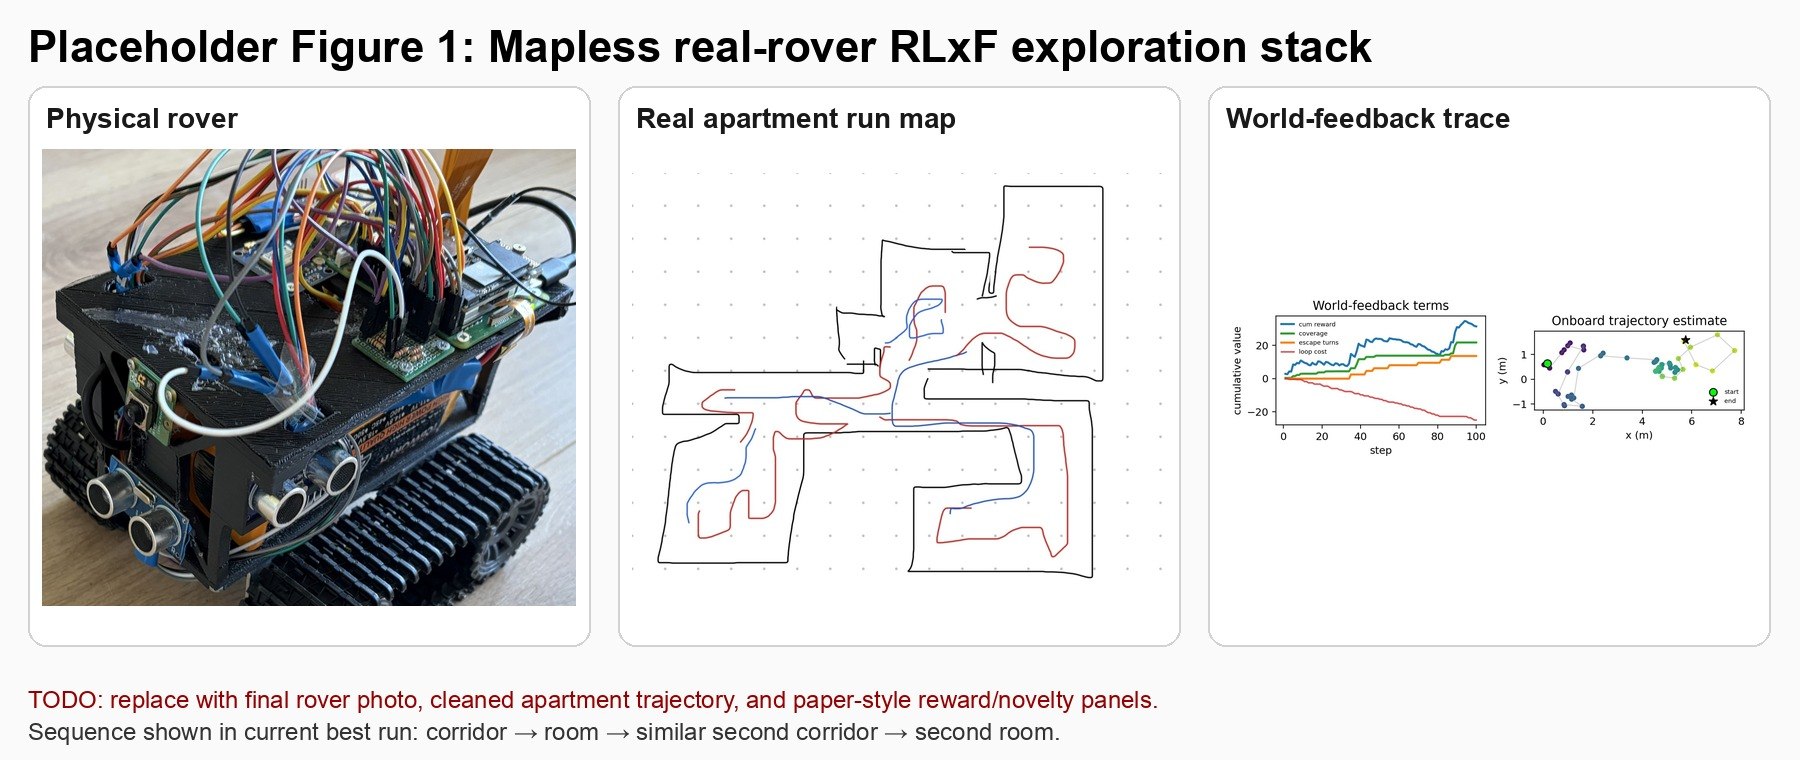
\includegraphics{data/hero_placeholder/figures/hero_placeholder.jpg}}
  \refstepcounter{figure}\label{fig:hero-placeholder}
  {\small \textbf{Figure~\thefigure: Placeholder --- get better images of this.} Real-rover RLxF exploration overview: physical platform, apartment-scale trajectory, and world-feedback reward traces. This temporary teaser sets the intended first-page feel before final photography and plotting.}
  \end{center}

  \vskip 0.15in
]

% this must go after the closing bracket ] following \twocolumn[ ...

% This command actually creates the footnote in the first column listing the
% affiliations and the copyright notice. The command takes one argument, which
% is text to display at the start of the footnote. The \icmlEqualContribution
% command is standard text for equal contribution. Remove it (just {}) if you
% do not need this facility.

% Use ONE of the following lines. DO NOT remove the command.
% If you have no special notice, KEEP empty braces:
\printAffiliationsAndNotice{}  % no special notice (required even if empty)
% Or, if applicable, use the standard equal contribution text:
% \printAffiliationsAndNotice{\icmlEqualContribution}

\section{Introduction}
Autonomous exploration is usually framed as mapping: estimate free space, detect frontiers, and plan to informative boundaries \citep{yamauchi1997frontier,thrun2005probabilistic}. This assumption is brittle on small low-cost robots with only monocular vision, short-range sensors, and noisy inertial measurements. In damaged buildings or rubble, the map may also change while the robot is operating.

We study \emph{mapless exploration from world feedback}. A physical rover learns online without external instrumentation, pre-built maps, or simulator pretraining. After each action, the only feedback is onboard: camera frames, range sensors, inertial response, executed motion, and recovery events. The environment supplies consequences; the designer specifies how to turn them into reward.

The central hypothesis is that learning should decide \emph{where to try next}, not raw motor PWM. A deterministic executor realizes the command near obstacles. Our strongest current abstraction is a relative heading followed by forward motion until the world, via front-range feedback, says to stop.

Intrinsic motivation is a natural reward source \citep{pathak2017curiosity,burda2019rnd,savinov2019episodic}, but real hardware exposes failure modes hidden in simulation: blur can look novel, wall contact can produce new pixels, and corridor loops can collect reward. We therefore gate novelty by executed motion and log penalties for recovery, zero-progress, and revisits.

This is an in-progress real-rover RLxF report. The policy is trained on hardware; saved trajectories are for auditing and ablations, not supervised pretraining. Evaluation uses quantities available to the robot and reviewer: successful motion, novel places, recovery frequency, and qualitative apartment coverage.

Our contribution is a minimal real-world benchmark and prototype stack: onboard RL, intrinsic visual memory, safety-gated local actions, and auditable world-feedback rewards.

\section{Methodology}

\begin{figure}[t]
  \centering
  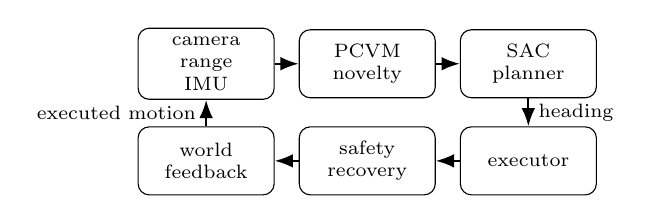
\begin{tikzpicture}[
    font=\scriptsize,
    box/.style={draw, rounded corners, align=center, minimum height=0.34in, minimum width=0.68in},
    arrow/.style={-Latex, thick}
  ]
    \node[box] (obs) {camera\\range\\IMU};
    \node[box, right=0.12in of obs] (pcvm) {PCVM\\novelty};
    \node[box, right=0.12in of pcvm] (sac) {SAC\\planner};
    \node[box, below=0.14in of sac] (exec) {executor};
    \node[box, left=0.12in of exec] (safety) {safety\\recovery};
    \node[box, left=0.12in of safety] (world) {world\\feedback};
    \draw[arrow] (obs) -- (pcvm);
    \draw[arrow] (pcvm) -- (sac);
    \draw[arrow] (sac) -- node[right]{heading} (exec);
    \draw[arrow] (exec) -- (safety);
    \draw[arrow] (safety) -- (world);
    \draw[arrow] (world) -- node[left]{executed motion} (obs);
  \end{tikzpicture}
  \caption{Current decoupled architecture. The Predictive Contextual Visual Memory (PCVM) module supplies novelty; SAC chooses a relative heading; the executor and safety layer determine what actually happens and return world feedback.}
  \label{fig:architecture-placeholder}
\end{figure}

\subsection{Problem setting}

At time $t$ the rover receives
\begin{equation}
o_t = (I_t, d_t, m_t, a_{t-1}, e_{t-1}),
\end{equation}
where $I_t$ is the camera image, $d_t$ range, $m_t$ inertial/proprioceptive state, $a_{t-1}$ the previous high-level action, and $e_{t-1}$ what the executor actually achieved. The policy selects a local guide $a_t$, not motor commands; the executor applies safety constraints and returns world feedback.

The goal is exploration under a fixed step budget, without a metric map or ground-truth pose. Dead-reckoned pose is only diagnostic.

\subsection{Local action abstraction}

The current action is a scalar relative heading
\begin{equation}
a_t \in [-1,1], \qquad \theta_t = \theta_{\max} a_t,
\end{equation}
with $\theta_{\max}=75^\circ$. The executor turns by $\theta_t$, then drives until the front sensor reaches a threshold or a max duration expires. This local, egocentric interface avoids global localization and discourages tiny dithering moves.

Other guides, such as short $(\theta,\rho)$ targets, fit the same framework. The key separation is intent from execution.

\subsection{Onboard novelty memory}

We call the current memory backend \emph{Predictive Contextual Visual Memory} (PCVM). It maps the frame and action context to $z_t$ and stores representative embeddings. Novelty is nearest-memory distance and/or RND-style prediction error \citep{burda2019rnd}:
\begin{equation}
n_t = \alpha \, \mathrm{dist}(z_t, \mathcal{M}_{t-1}) + \beta \, \|f_{\mathrm{pred}}(I_t)-f_{\mathrm{target}}(I_t)\|_2^2,
\end{equation}
where $\mathcal{M}_{t-1}$ is memory and $f_{\mathrm{target}}$ is fixed. Distant embeddings create or update memory representatives.

The final encoder is not fixed; we have tested lightweight CNNs, recurrent path-conditioned memory, and frozen backbones. The framework only requires onboard novelty estimates.

\subsection{World-feedback reward}

Novelty alone is insufficient: the robot can see new pixels while stuck. Reward combines perceptual novelty with execution feedback:
\begin{align}
r_t ={}& r_t^{+} - r_t^{-}, \\
r_t^{+} ={}& w_n\,\mathbb{1}[M_t] n_t
       + w_c C_t
       + w_d \Delta s_t
       + w_s S_t, \\
r_t^{-} ={}& \lambda_r R_t
       + \lambda_0 Z_t
       + \lambda_l L_t
       + \lambda_o O_t .
\end{align}
Here $M_t$ gates novelty by motion, $C_t$ denotes cluster/coverage expansion, $S_t$ safe motion, $\Delta s_t$ executed distance, and $R_t,Z_t,L_t,O_t$ recovery, zero-forward, revisit, and obstacle penalties.

Each term is logged separately, so scalar reward can be audited against video. This exposed early over-rewarding of corridor loops and motivated loop-aware penalties.

\subsection{Training and data usage}

We currently use SAC \citep{haarnoja2018sac}. Replay is populated online from rover experience. Safety can clip execution, and the policy receives the executed-action feedback.

Saved manual/autonomous runs are used only for reward auditing, memory diagnostics, and figures, not policy pretraining.

\subsection{Evaluation protocol}

Evaluation uses short autonomous episodes with successful-forward fraction, recoveries, zero-progress, dead-reckoned spread, and frame review. Frozen runs serve as reward-alignment diagnostics.

\section{Preliminary Real-Rover Experiments}

\paragraph{Use case framing.}
The motivating deployment is an unknown and changing indoor structure, e.g. a small rescue rover entering damaged buildings or rubble. The robot cannot rely on a precomputed map, but it can evaluate the consequences of its actions through onboard feedback.

\paragraph{Representative run.}
Figure~\ref{fig:hero-placeholder} includes reward and trajectory panels from a 100-step continuation run. The human-observed sequence was corridor $\rightarrow$ room $\rightarrow$ visually similar second corridor $\rightarrow$ second room. The third segment receives less novelty, plausibly because the apartment has an X-shaped corridor geometry with overlapping views. This is qualitative until repeated runs and ablations are complete.

\begin{figure}[t]
  \centering
  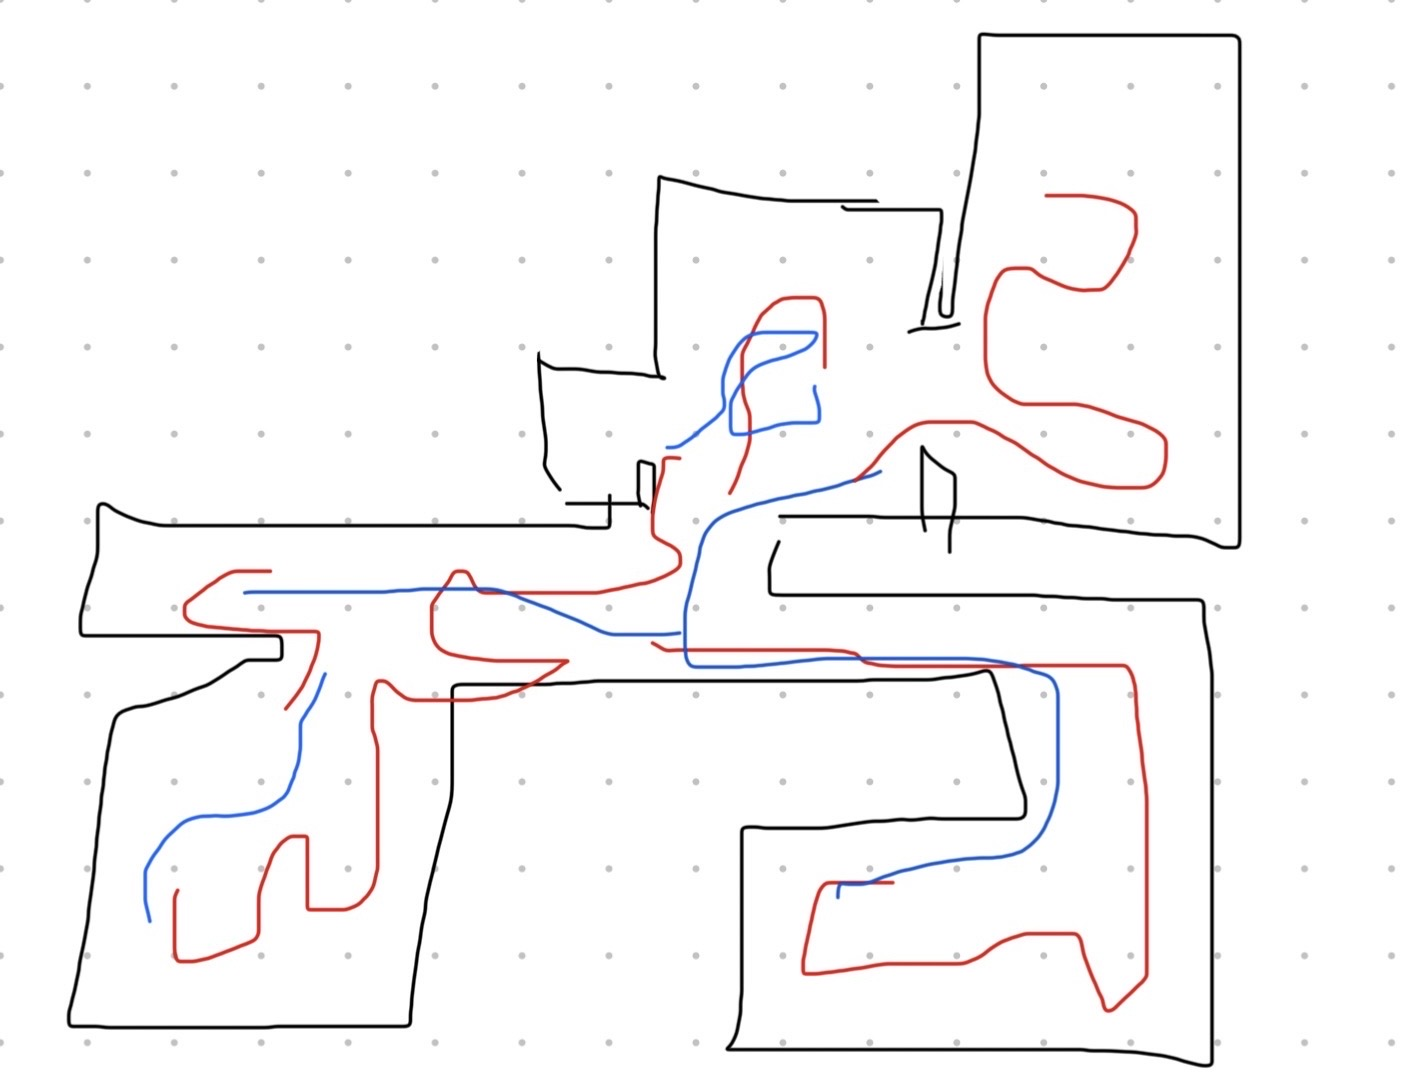
\includegraphics[width=0.48\textwidth]{data/hero_placeholder/raw/final_run_map.jpg}
  \caption{Placeholder apartment/run map. This half-column figure is only for layout exploration; replace with a cleaned schematic or manually annotated map before submission.}
  \label{fig:placeholder-apartment-map}
\end{figure}

The run scored $+31.5$ over 100 actions, traveled $20.3\,$m, reached $5.7\,$m net displacement, and expanded the dead-reckoned box to $22.3\,\mathrm{m}^2$. It still had two contact/stall events and many recoveries, so the controller is not solved; the result only suggests that the action/reward interface can produce room-to-room exploration.

\clearpage

\begin{table*}[!t]
  \centering
  \caption{Placeholder ablation and benchmark matrix. Empty cells mark measurements to fill after repeated runs.}
  \label{tab:placeholder-benchmarks}
  \small
  \resizebox{\textwidth}{!}{%
  \begin{tabular}{lcccccc}
    \toprule
    System / ablation & Rooms & Travel & Contacts & Reward & Notes & Status \\
    \midrule
    Short local target PCVM &  &  &  &  &  & old baseline \\
    Theta-front PCVM &  &  &  &  &  & current baseline \\
    Theta-front + coverage reward &  &  &  &  &  & current run \\
    No surprise term &  &  &  &  &  & planned \\
    Executed-action memory &  &  &  &  &  & planned \\
    Human WASD reference &  &  &  &  &  & reference \\
    \bottomrule
  \end{tabular}}
\end{table*}

\section{Ablations}

\paragraph{Draft notes from current rover runs.}
Current evidence points first to action interface: short local targets produced timid motion, while relative-heading plus world-bounded execution reached multiple rooms. This motivates a fixed-distance target vs. drive-until-front ablation. A second ablation is requested-action memory vs. executed-action memory, because safety clipping and recovery change what physically happened. A third is surprise on/off: transition error may capture useful unmodeled outcomes, but may also reward blur, noise, or collision artifacts.

\paragraph{Reward-alignment drafts.}
The coverage reward was introduced after visual review showed that a two-room run scored lower than a corridor loop. Future ablations should rank frozen runs by human labels: corridor loop $<$ corridor+one-room $<$ corridor+two-room. This allows reward tuning before spending hardware time.

\paragraph{Architecture drafts.}
The current PCVM module still aliases similar rooms/corridors. We plan to compare lightweight CNN features, frozen pretrained encoders, and dual path/visual memory while keeping the same theta-front executor.

\section{Conclusion \& Future Work}

This draft supports a narrow claim: decoupled planning and terrain-adaptive execution can produce useful real-rover exploration from onboard world feedback. Future work is safety-aware reward, separate sensor/safety monitors for low-cost hardware, and stronger pretrained visual encoders for room-level novelty.


% In the unusual situation where you want a paper to appear in the
% references without citing it in the main text, use \nocite
% \nocite{langley00}

\clearpage
\bibliography{example_paper}
\bibliographystyle{icml2026}

\clearpage
\appendix
\section{Appendix Placeholder}

This appendix will contain extended run sheets, additional frame grids, reward-audit details, and repeated-run ablations. The main paper target is four pages before references and appendix.

\end{document}

% This document was modified from the file originally made available by
% Pat Langley and Andrea Danyluk for ICML-2K. This version was created
% by Iain Murray in 2018, and modified by Alexandre Bouchard in
% 2019 and 2021 and by Csaba Szepesvari, Gang Niu and Sivan Sabato in 2022.
% Modified again in 2023 and 2024 by Sivan Sabato and Jonathan Scarlett.
% Previous contributors include Dan Roy, Lise Getoor and Tobias
% Scheffer, which was slightly modified from the 2010 version by
% Thorsten Joachims & Johannes Fuernkranz, slightly modified from the
% 2009 version by Kiri Wagstaff and Sam Roweis's 2008 version, which is
% slightly modified from Prasad Tadepalli's 2007 version which is a
% lightly changed version of the previous year's version by Andrew
% Moore, which was in turn edited from those of Kristian Kersting and
% Codrina Lauth. Alex Smola contributed to the algorithmic style files.
